\documentclass[letterpaper,12pt,fleqn]{article}
\usepackage{matharticle}
\usepackage{mathtools}
\pagestyle{plain}
\begin{document}

\begin{center}
\Large Math-19 Homework \#2 Solutions
\end{center}

\vspace{0.5in}

\underline{Problems}

\begin{enumerate}
\item Let:
\begin{eqnarray*}
P &\coloneqq& 0\ \mbox{is a positive number} \\
Q &\coloneqq& 2\ge2 \\
R &\coloneqq& \forall n,m\in\mathbb{N}, n+m\in\mathbb{N} \\
\end{eqnarray*}
Determine whether the following (compound) statements are true or false:

\begin{tabular}{|c|c|l|}
  \hline
  Statement & T/F & comment \\
  \hline
  P & F & Zero is neither positive nor negative. \\
  \hline
  Q & T & $\ge$ means ``greater than OR equal to''. \\
  \hline
  R & T & This is closure of the natural numbers under addition. \\
  \hline
  not P & T & not F = T \\
  \hline
  not Q & F & not T = F \\
  \hline
  not R & F & not T = F \\
  \hline
  P and Q & F & F and T = F \\
  \hline
  P and R & F & F and T = F \\
  \hline
  Q and R & T & T and T = T\\
  \hline
  P or Q & T & F and T = T \\
  \hline
  P or R & T & F and T = T \\
  \hline
  Q or R & T & T and T = T \\
  \hline
\end{tabular}

\bigskip

\item Convert $10.2\overline{45}$ to rational form.

  Let $x=10.2\overline{45}$. We want $x=\frac{p}{q}$ for $p,q\in\Z$ and
  $q\ne0$.
  
  Capture all of the fixed digits:
  \[10x=102.\overline{45}\]

  Now, capture all of the fixed digits, and one set of repeating digits.
  \[1000x=10245.\overline{45}\]

  Solve for $x$ by subtracting the first equation from the second:
  \begin{eqnarray*}
    990x &=& 10143 \\
    x &=& \frac{10143}{990}
  \end{eqnarray*}
  You can reduce, but not required here.
  \[x=\frac{1127}{110}\]
  
\bigskip

\item Let:
\begin{eqnarray*}
A &=& \mbox{the set of all positive real numbers} \\
B &=& \mbox{the set of real numbers between -3 (exclusive) and 3 (inclusive)} \\
\end{eqnarray*}

\newcommand{\tick}[1]{\draw (#1,0.1) -- (#1,-0.1)}
\newcommand{\ocirc}[1]{\draw (#1,0) circle [radius=0.1]}
\newcommand{\ccirc}[1]{\draw [fill=black] (#1,0) circle [radius=0.1]}

\begin{enumerate}
\item Graph each set on the real number line.

  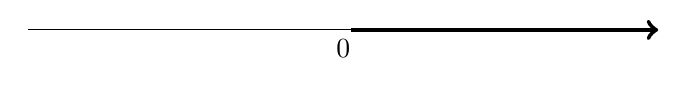
\begin{tikzpicture}
    \draw (-4,0) -- (4,0);
    \tick{0};
    \ocirc{0};
    \draw [->, ultra thick] (0.1,0) -- (4,0);
    \node [below] at (0,0) {0};
  \end{tikzpicture}

  
\begin{tikzpicture}
    \draw (-4,0) -- (4,0);
    \tick{-3};
    \tick{3};
    \ocirc{-3};
    \ccirc{3};
    \draw [ultra thick] (-2.9,0) -- (3,0);
    \node [below] at (-3,0) {-3};
    \node [below] at (3,0) {3};
  \end{tikzpicture}
  
\item Represent each set using set-builder notation.
\[A=\{x\in\R\mid x>0\}\]
\[B=\{x\in\R\mid -3<x\le3\}\]

\item Represent each set using interval notation.
\[A=(0,\infty)\]
\[B=(-3,3]\]

\item Graph $A\cup B$ and represent it in interval notation.

  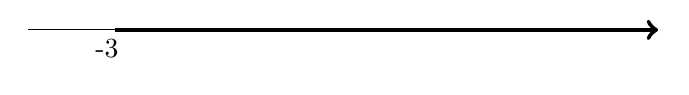
\begin{tikzpicture}
    \draw (-4,0) -- (4,0);
    \tick{-3};
    \ocirc{-3};
    \draw [ultra thick,->] (-2.9,0) -- (4,0);
    \node [below] at (-3,0) {-3};
  \end{tikzpicture}
  \[A\cup B=(-3,\infty)\]
  
\item Graph $A\cap B$ and represent it in interval notation.

  
\begin{tikzpicture}
    \draw (-4,0) -- (4,0);
    \tick{0};
    \tick{3};
    \ocirc{0};
    \ccirc{3};
    \draw [ultra thick] (0.1,0) -- (3,0);
    \node [below] at (0,0) {0};
    \node [below] at (3,0) {3};
  \end{tikzpicture}
  \[A\cap B=(0,3]\]

\item Graph $A-B$ and represent it in interval notation.

  \begin{tikzpicture}
    \draw (-4,0) -- (4,0);
    \tick{3};
    \ocirc{3};
    \draw [ultra thick,->] (3.1,0) -- (4,0);
    \node [below] at (3,0) {3};
  \end{tikzpicture}
  \[A-B=(3,\infty)\]
\end{enumerate}

\item A careful solution of $4(x+2)=11$ is given below. Give the rationale for
each step from the ten real number rules (AC,AA,A0,AI,MC,MA,M1,MI,LD,RD) and
the additional rules (SUB,WD).

\begin{tabular}{ll}
$4(x+2)=11$ & \\
$4x+8=11$ & LD \\
$(4x+8)-8=11-8$ & CAN \\
$(4x+8)-8=3$ & SUB \\
$4x+(8-8)=3$ & AA \\
$4x+0=3$ & AI \\
$4x=3$ & A0 \\
$\frac{1}{4}(4x)=\frac{1}{4}(3)$ & CAN \\
$\frac{1}{4}(4x)=\frac{3}{4}$ & SUB \\
$(\frac{1}{4}4)x=\frac{3}{4}$ & MA \\
$1x=\frac{3}{4}$ & MI \\
$x=\frac{3}{4}$ & M1 \\
\end{tabular}

\bigskip

\item Consider the statement: $\forall\,a,b\in\R,|a-b|=|b-a|$
  \begin{enumerate}
  \item Give a careful proof of this statement. You will need to use one of
    the distributive rules (hint: factor out a -1), one of the properties in
    the box at the top of page 9 of your textbook, and the definition of
    absolute value.

    \begin{tabular}{ll}
      $\abs{a-b}=\abs{-(b-a)}$ & Prop of Neg \#6 \\
      $\abs{a-b}=\abs{(-1)(b-a)}$ & Prop of Neg \#1 \\
      $\abs{a-b}=\abs{-1}\abs{b-a}$ & Prop of AV \#3 \\
      $\abs{a-b}=1\cdot\abs{b-a}$ & Def of AV \\
      $\abs{a-b}=\abs{b-a}$ & M1 \\
    \end{tabular}

    or:

    \begin{tabular}{ll}
      $\abs{a-b}=\abs{-(-a)-b}$ & Prop of Neg \#2 \\
      $\abs{a-b}=\abs{-(-a+b)}$ & Prop of Neg \#5 \\
      $\abs{a-b}=\abs{-(b+(-a))}$ & AC \\
      $\abs{a-b}=\abs{-(b-a)}$ & Definition of Subtraction \\
      $\abs{a-b}=\abs{b-a}$ & Prop of AV \#2 \\
    \end{tabular}

  \item What does this statement mean (what are the semantics)? (Hint: think
    distance)

    The distance between $a$ and $b$ is the same as the distance between
    $b$ and $a$.
  \end{enumerate}
\end{enumerate}
\end{document}
